\documentclass[11pt]{article}
\usepackage[utf8]{inputenc}

\usepackage{hyperref}
\usepackage{wrapfig}
\usepackage{amsmath}
\usepackage{minted}
\usepackage{color}
\usepackage{svg}
\usepackage{graphicx}
\usepackage{fancyhdr}
\usepackage{natbib}

\bibliographystyle{humannat}

\graphicspath{ {./images/} }
\setlength{\tabcolsep}{10pt}
\setlength{\headheight}{15pt}

\providecommand{\shortcite}[1]{\cite{#1}}

\title{A visualiser for $\lambda$-terms as rooted 3-valent maps}
\author{George Kaye}
\date{March 2019}

\makeatletter

\pagestyle{fancy}
\fancyhf{}
\fancyhead[R]{\textsl{\rightmark}}
\fancyfoot[C]{\thepage}

\renewcommand{\footrulewidth}{0.5pt}

\begin{document}

\input{titlepage.tex}

\tableofcontents

\newpage

\section{Abstract}
\label{sec:abstract}
Todo

\newpage

\section{Acknowledgements}
\label{sec:acks}
Todo


\newpage

\section{Introduction}
\label{sec:intro}

This report details the development of a set of tools to aid in the research of the topological properties of $\lambda$-terms when they are represented as rooted maps.

\subsection{\texorpdfstring{$\lambda$}{lambda}-term visualiser}

Drawing $\lambda$-terms maps by hand can be quite time-consuming, especially for large terms. The first tool can generate maps for $\lambda$-terms from user input, in addition to providing interesting properties such as crossings. By visualising the $\lambda$-terms it can become much easier to understand the structure of more complex structures implemented in the $\lambda$-calculus (such as pairs).

The visualiser also has functionality relating to the normalisation of terms. The $\beta$-redexes contained within the term are listed, and by clicking on these the user can reduce the term to its normal form (if one exists). A normalisation graph can also be generated, which can also be interesting to examine.

\subsection{\texorpdfstring{$\lambda$}{lambda}-term gallery}
When studying properties of $\lambda$-terms, it can be useful to generate terms and look for interesting properties shared between terms and their maps. However it can be tricky to come up with terms with certain properties (such as terms containing a certain amount of subterms) on the fly. The $\lambda$-term gallery can generate all terms of a certain size and free variables, with the ability to filter based on properties such as crossings or $\beta$-redexes. This makes testing conjectures a much easier process.

From the gallery, the user can inspect the generated terms using the visualiser, with the same functionality present as detailed above.

\begin{figure}
    \centering
    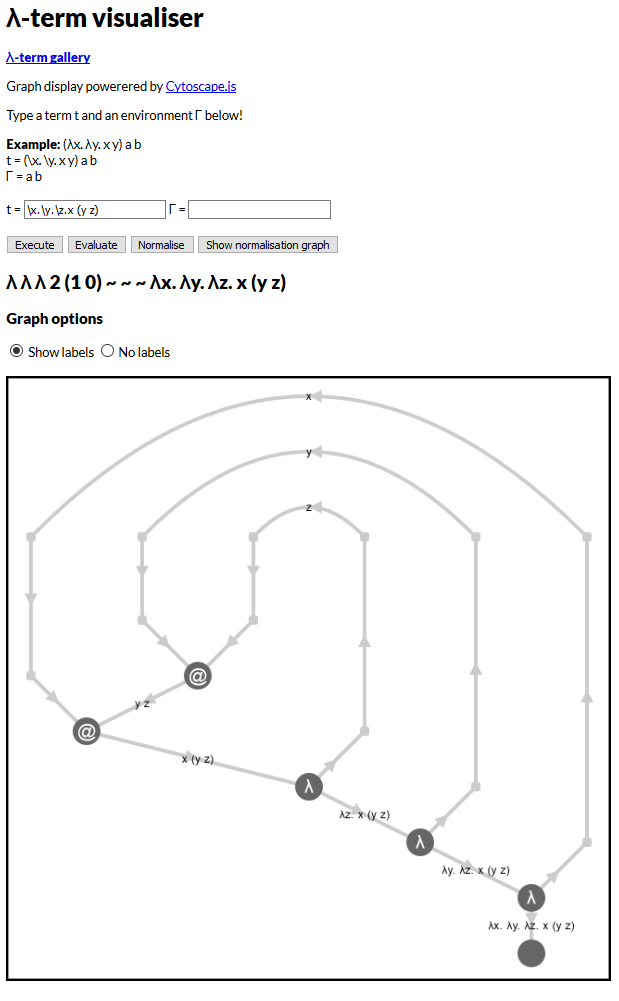
\includegraphics[scale=0.3]{visualiser}
    \caption{The $\lambda$-term visualiser, displaying the map for the term $\lambda x. \lambda y. \lambda z. x \, (y \, z)$, along with some statistics on the right.}
    \label{fig:visualiser}
\end{figure}

\begin{figure}
    \centering
    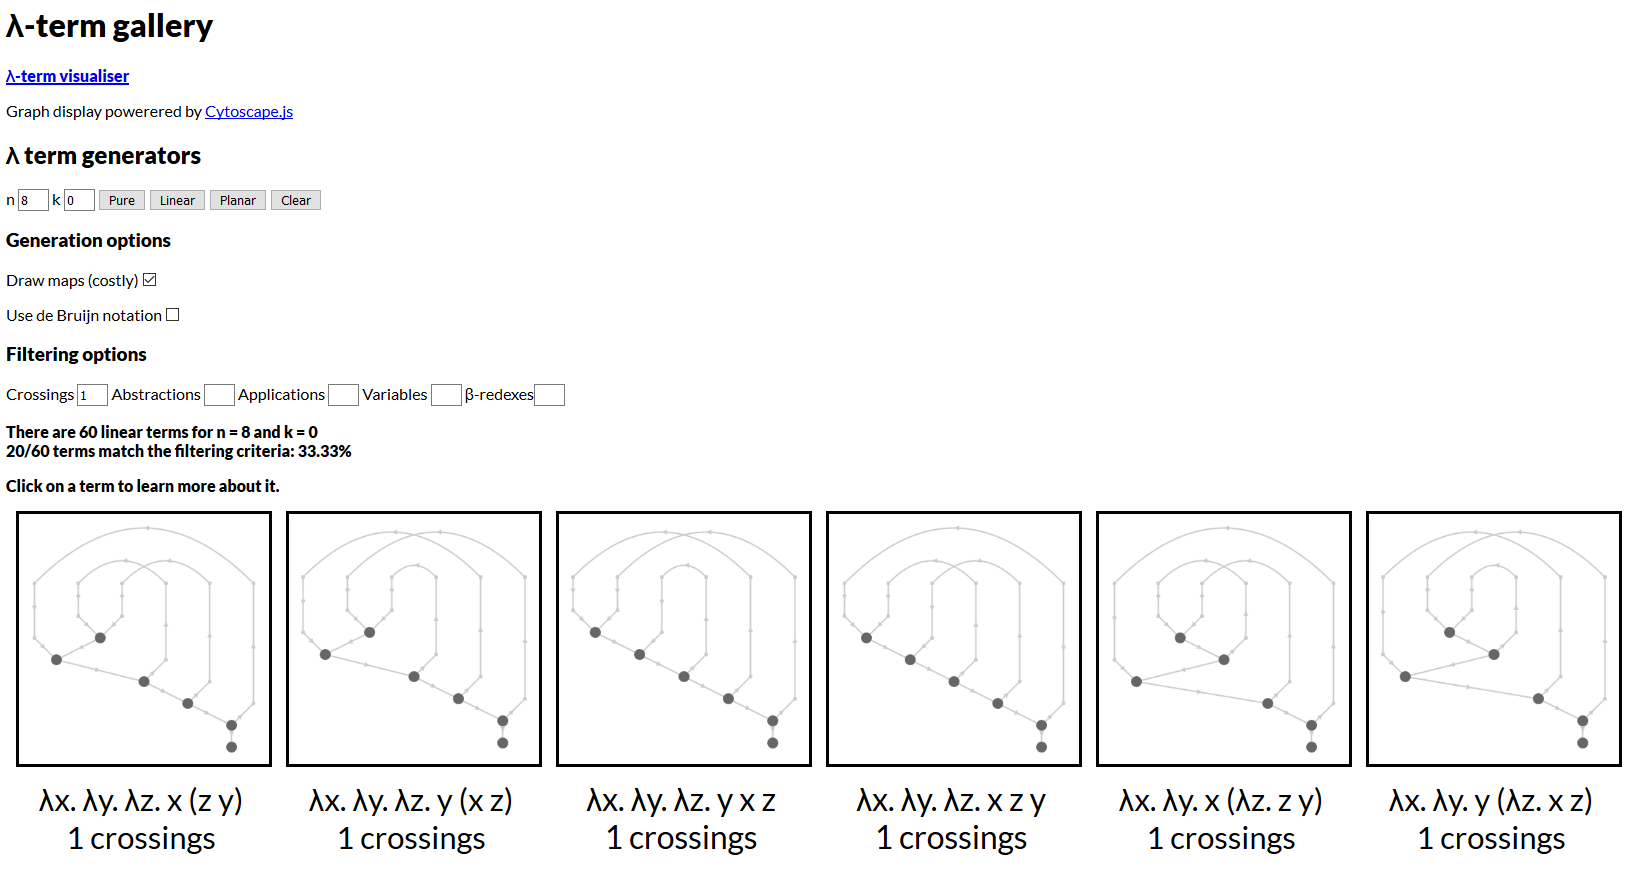
\includegraphics[scale=0.3]{gallery}
    \caption{The $\lambda$-term gallery, displaying all closed linear terms of size 5.}
    \label{fig:gallery}
\end{figure}

\newpage

\section{Background}
\label{sec:background}

\subsection{The \texorpdfstring{$\lambda$}{lambda}-calculus}
The $\lambda$-calculus is a model of computation where programs are represented by variable abstraction and function application. It is the basis of all functional programming languages. This section will cover some concepts and terminology that will be used in the remainder of the report.

\subsubsection{Definitions}
\label{sec:defs}

The simplest terms in the $\lambda$-calculus ($\lambda$-terms) are just \textbf{variables} ($x, y, z, ...$). More complex terms can be created using the operations of \textbf{abstraction} ($\lambda x. T$) and \textbf{application} $(T_1 T_2)$. For clearer notation, applications are left-associative and abstractions extend as far to the right as possible:
%
\begin{align*}
    x \, y \, z &\equiv (x \, y) \, z \\
    \lambda x. x \, \lambda y. y &\equiv (\lambda x. x \, (\lambda y. y))
\end{align*}
%
Variables in the $\lambda$-calculus can be \textbf{bound} or \textbf{free}. A variable is bound if it is inside the scope of a corresponding $\lambda$-abstraction (it is a local variable), or free otherwise. In $\lambda x. x \, y$, the $x$ is bound but the $y$ is free. A $\lambda$-term with no free variables is called a \textbf{closed term}. Two $\lambda$-terms are said to be \textbf{$\alpha$-equivalent} if the only difference between them is the names of their bound variables -- for example, $\lambda x. x$ and $\lambda y. y$ are $\alpha$-equivalent. The process of renaming bound variables is known as \textbf{$\alpha$-conversion}:
%
$$\lambda x. T \to_\alpha \lambda y. T[x \mapsto y]$$
%
To avoid ambiguity between $\alpha$-equivalent terms, we can use \textbf{de Bruijn notation}. Rather than using explicit variable names, each variable is instead represented by how 'far away' the corresponding abstraction is. For example, $\lambda x. \lambda y. \lambda z. x \, y \, z$ can be written as $\lambda\lambda\lambda \, 2 \, 1 \, 0$. This eliminates the need for $\alpha$-conversion and makes it far more efficient to determine equality of $\lambda$-terms.

$\lambda$-terms contain a number of \textbf{subterms}, defined as:
%
\begin{align*}
    subterms(x) &= 1 \\
    subterms(\lambda x. T) &= 1 + subterms(T) \\
    subterms(T_1 T_2) &= 1 + subterms(T_1) \, + \, subterms(T_2)
\end{align*}

\subsubsection{\texorpdfstring{$\beta$}{Beta}-reduction}

Program execution in the $\lambda$-calculus is performed through \textbf{$\beta$-reduction} -- applying functions to their arguments. A term of the form $(\lambda x. T_1) \, T_2$ is called a \textbf{$\beta$-redex} and can be $\beta$-reduced as follows:
%
$$(\lambda x. T) \, u \to_\beta T[x \mapsto u]$$
%
Repeatedly performing $\beta$-reduction on a term until it contains no $\beta$-redexes is known as \textbf{normalisation}. A term with no $\beta$-redexes is in its \textbf{normal form}. All $\lambda$-terms have a unique normal form. If there are multiple $\beta$-redexes in a term, the order they are reduced in does not matter -- the same normal form will be reached. This is known as the \textbf{Church-Rosser theorem} (\cite{churchrosser}). However, for some pure terms the normal form is not computable, as attempts to reduce them will lead to a loop. One well-known example is the $\Omega$ term:
%
$$ \Omega = (\lambda x. x \, x)(\lambda x. x \, x) \rightarrow_\beta (x \, x)[x \mapsto (\lambda x. x \, x)] \equiv (\lambda x. x \, x)(\lambda x. x \, x) \equiv \Omega $$
%
When it is possible to get stuck in one of these normalisation loops, the order of reduction can actually matter. as shown by the example below, where reducing redex 1 leads to a new term whereas redex 2 leads to the same term:
%
$$ T = \underbrace{(\lambda x. \lambda y. x) \, a}_\text{redex 1} \, \underbrace{((\lambda x. x \, x) (\lambda x. x \, x))}_\text{redex 2} $$

$$ T \rightarrow_{\beta1} (\lambda y. a)((\lambda x. x \, x)(\lambda x. x \, x)) $$
%
$$ T \rightarrow_{\beta2} (\lambda x. \lambda y. x) \, a \, ((\lambda x. x \, x)(\lambda x. x \, x))$$
%
The choice of which redex to reduce is related to \textbf{evaluation strategies}. Choosing the \textbf{outermost reduction} corresponds to \textbf{normal order} evaluation, in which arguments are substituted into a function before they are evaluated. Conversely, chosing the \textbf{innermost reduction} corresponds to \textbf{applicative order} evaluation, where arguments are fully evaluated before being applied to functions. Always choosing the outermost reduction is guaranteed to find the normal form if it exists. This is not the case for choosing the innermost reduction since an argument that is not used in a function could contain a normalisation loop.

The process of normalisation can be represented by \textbf{normalisation graphs}, which show the various paths between a $\lambda$-term and its normal form. An example of normalisation graphs can be seen in Figure \ref{fig:normgraphs} and \ref{fig:normgraphs2}.

\begin{figure}
    \centering
    \includegraphics{reduction}
    \caption{An example of two normalisation graphs, showing the steps of reduction taken for the terms $\lambda x. (\lambda y \, x) (\lambda z. z)$ and $\lambda x. (\lambda y. y) ((\lambda z. z) \, x)$ to reach their normal forms. Note that the diverging paths in the right example still lead to the same normal form, as stated by the Church-Rosser theorem.}
    \label{fig:normgraphs}
\end{figure}

\begin{figure}
    \centering
    \includegraphics[scale=0.4]{norm2}
    \caption{Normalisation graphs, showing the steps of reduction taken for the terms for the terms $(\lambda x. x \, x)(\lambda x. x \, x)$ and $(\lambda x. \lambda y. x) \, a \, ((\lambda x. x \, x)(\lambda x. x \, x)$, showing the normalisation loops that can occur.}
    \label{fig:normgraphs2}
\end{figure}

\subsubsection{Fragments of the \texorpdfstring{$\lambda$}{lambda}-calculus}
The \textbf{pure $\lambda$-calculus} contains all terms formed from combining variables, abstractions and applications. However we can restrict ourselves to smaller \textbf{fragments} of the $\lambda$-calculus. The \textbf{linear $\lambda$-calculus} is a subset of the pure $\lambda$-calculus containing terms in which variables are used exactly once, and the \textbf{planar $\lambda$-calculus} is a subset of the linear $\lambda$-calculus in which variables are used in the order they are abstracted in. Linear and planar $\lambda$-terms have special properties relating to maps, which will be covered in the next section.

\begin{table}
    \centering
    \begin{tabular}{|c|c|c|c|}
        \hline
        \textbf{Term} & \textbf{Pure} & \textbf{Linear} & \textbf{Planar} \\
        \hline
        $\lambda x. x$ & Yes & Yes & Yes \\
        \hline
        $\lambda x. (\lambda y. y) \, x$ & Yes & Yes & Yes \\
        \hline
        $\lambda x.\lambda y. x \, y$ & Yes & Yes & Yes \\
        \hline
        $\lambda x. \lambda y. y \, x$ & Yes & Yes & No \\
        \hline
        $\lambda x. x \, x$ & Yes & No & No \\
        \hline
    \end{tabular}
    \caption{Examples of terms in various fragments of the $\lambda$-calculus.}
    \label{tab:fragments}
\end{table}

\subsection{Graphs and maps}

\begin{figure}
    \centering
    \includesvg{maps}
    \caption{These two diagrams represent the same graph but two distinct maps (the ordering of edges around the point on the circle is changed). Adapted from Lando, Zvonkin {\cite{graphs}}}
    \label{fig:maps}
\end{figure}

In graph theory, a \textbf{graph} is a set of nodes and edges that link pairs of nodes. When these graphs are \textbf{embedded} onto a surface they are called \textbf{maps}. Unlike graphs, the order of edges around a node is important for maps, and the same graph can be represented as many different maps (an example is shown in Figure \ref{fig:maps}). A map has a \textbf{genus} which is how many 'holes' the surface it is embedded into has. \textbf{Planar maps} are maps with no crossings of edges -- they have a genus of 0. 

In this project we are particularly interested with \textbf{rooted 3-valent maps}. The \textbf{valency} of a node is how many edges connect to it - maps where all of the nodes have a valency of 3 are called \textbf{3-valent}. We can make a \textbf{rooted map} by adding a 'special' node (the \textbf{root}) that connects to the map at one point, as shown in Figure \ref{fig:trivalentrooted}.

\begin{figure}
    \centering
    \includegraphics[scale=0.3]{torus}
    \caption{An example of how a graph with crossings can be embedded onto a torus. From \shortcite{zeil4ct}.}
    \label{fig:torus}
\end{figure}

\begin{figure}
    \centering
    \includesvg[scale=0.5]{trivalentrooted}
    \caption{A 3-valent map, and the same map but rooted (root indicated by the white node)}
    \label{fig:trivalentrooted}
\end{figure}

We can represent $\lambda$-terms as maps. Abstractions and applications are represented as nodes, as shown in Figure \ref{fig:absapp}. With the addition of a root to represent the start of the term, these nodes can be combined to create a rooted map, as shown in Figure \ref{fig:trivalentrooted}.

Viewing these $\lambda$-term maps can be interesting for many reasons. We can tell which terms are linear since their corresponding maps are 3-valent -- abstracted variables are only used once. Planar terms correspond to planar graphs with no crossings.

\begin{figure}
    \centering
    \includegraphics[scale=0.7]{absapp}
    \caption{An abstraction and an application, represented as nodes of a map.}
    \label{fig:absapp}
\end{figure}

\begin{figure}
    \centering
    \includegraphics[scale=0.8]{lambdatermandgraph}
    \caption{A representation of the term $\lambda x. \lambda y. \lambda z. x \, (y \, z)$ as a rooted 3-valent map, without and with node labels. From \protect\cite{zeiljfp}.}
    \label{fig:lambdatermandgrapht}
\end{figure}

\newpage

\section{Features}


\section{Design}
\label{sec:design}

The two tools 

\subsection{\texorpdfstring{$\lambda$}{Lambda}-term visualiser}


\subsection{\texorpdfstring{$\lambda$}{Lambda}-term gallery}



\newpage

\section{Implementation}
\label{sec:implementation}

This section will cover the implementation of the tools, and issues that rose.

\subsection{Language}
To implement the tools, I decided to use \texttt{Javascript}. This was so the tools could be distributed as 'web apps' and hosted on a website rather than having to be downloaded and relying on any dependencies.

\subsection{Implementing the \texorpdfstring{$\lambda$}{lambda}-calculus in \texttt{Javascript}}
The first part of developing the project was to implement the $\lambda$-calculus in \texttt{Javascript}, as a basis for the rest of the project to build on. The implementation partially based on the \texttt{ML} examples developed by \cite{pierce}. Variables are stored as de Bruijn indices -- this means that it is trivial to tell if terms are identical without having to perform $\alpha$-conversion. Abstractions and applications are constructed as combinations of subterms. Functionality was added later in the project so that terms can be associated with an \textbf{alias} to save time when writing out large expressions (for example, the alias \texttt{id} for the identity function $\lambda x. x$). An example of how terms can be represented can be seen in Figure \ref{fig:implementation}.

\begin{figure}
    \begin{minted}[frame=lines]{js}
    const y = new LambdaVariable(0);     
    const x = new LambdaVariable(1);      
    const app = new LambdaApplication(y, x);  
    const abs1 = new LambdaAbstraction(app, 'y');    
    const abs2 = new LambdaAbstraction(abs, 'x', 'swap'); 
    
    abs2.prettyPrint(); // prints \ \ 0 1
    \end{minted}
    \caption{How the function $swap = \lambda x. \lambda y. y \, x$ can be constructed in the \texttt{Javascript} implementation.}
    \label{fig:implementation}
\end{figure}

Since terms often contain free variables, a class to represent the context of a term was also created. This was effectively a wrapper for an array that contained the labels of terms currently in the context, with some extra methods to make manipulating it easier, such as determining a label from a given de Bruijn index. 

Printing the $\lambda$-terms proved to be more nuanced than expected. While the de Bruijn representation of a term is constant and easy to print, it is not very readable (especially in large terms) -- traditional labelled terms are much more intuitive. Originally variables stored a 'label' that could be printed instead of the index, but this proved to be quite buggy and often variables and their corresponding abstractions would display different labels (e.g. after $\alpha$-conversion). To fix this, labels were restricted to just abstractions, and when printing these labels would be added to a context. When the variables were to be printed, the index of the term would be looked up in the context and the appropriate label retrieved. This would ensure consistency (and subsequently correctness) throughout the term. 

When implementing the normalisation functionality, it became apparent that some sort of $\alpha$-conversion would still need to be implemented to avoid clashes of variables in the printed labels. A function was implemented to generate a 'canonical' set of labels, to ensure that each variable name was only used once in the term. For example, the term $(\lambda d. (\lambda h. h \, d) \, h) \, g$ with free variables $h$ and $g$ would be $\alpha$-converted to $\lambda x. (\lambda y. y \, x) \, a) \, b$. This would also be used when generating normalisation graphs later on -- redexes that led to $\alpha$-equivalent terms would have a consistent set of labels rather than juggling many different representations.

\subsection{Parsing terms from user input}
Initially the parser would iterate through the user input one character at a time, making note of 'special' characters (e.g. a backslash to represent a $\lambda$-abstraction, or an opening bracket to indicate the start of a subterm). It would then create the $\lambda$-term objects as it went from left to right. However the original parsing algorithm grew quite confusing, as it had to keep track of many different states (e.g. if an abstraction was in progress), and in practice elements could be more than one character long (such as longer variable names).

To make the process more intuitive, parsing was split into two distinct parts: an initial tokenising phase where the input would be split into the different tokens (e.g. $\lambda var. (\lambda y. y) \, var \implies$ \texttt{[\textbackslash,var,(,\textbackslash,y,),var)]}), and the parsing phase where these tokens would be formed into actual $\lambda$-terms. The benefit of tokenising first is that syntax errors (such as mismatched brackets or missing abstraction variables) are caught first, and the parser can iterate over tokens without having to worry about malformed terms. This also means that the parsing process is consistent even if variable names are longer than one character, as the labels can be stored as one token. 

This means that the 'special characters' the parser needs to check for are \texttt{(} and \texttt{)} for subterms, and \texttt{\textbackslash} for abstractions. Everything else is a variable, and adjacent tokens/subterms represent applications. To extend the parser to handle aliases, all that had to be added was to check tokens against the list of existing aliases, and use the corresponding function body if one existed.

\subsection{Drawing the terms}

To create the elements in the maps, the term is traversed recursively and new node objects are created when encountering an abstraction or application, with an edge leading to the previous parent node. When a variable is found, the appropriate edge is created between the parent node and the corresponding abstraction node. The array of map elements is then passed to the Cytoscape API which then generates the map.

\begin{figure}
    \centering
    \includegraphics[scale=0.17]{maps}
    \caption{How the map for the term $\lambda x. \lambda y. \lambda z. x \, (y \, z)$ evolved over time. Maps 1 and 2 are incorrect due to too many crossings, Maps 3 is correct but not aesthetically pleasing, Map 4 is the final (correct) version.}
    \label{fig:drawn_maps}
\end{figure}

\begin{figure}
    \centering
    \includegraphics[scale=0.17]{maps2}
    \caption{How the map for the term $\lambda x. \lambda y. x \, (\lambda a. \lambda b. b \, a) \, y$ evolved over time. Maps 1 is incorrect due to a lack of crossings, Map 2 is incorrect due to too many crossings, Map 3 is not only incorrect due to too many crossings but is also very hard to decipher, Map 4 is the final (correct) version.}
    \label{fig:drawn_maps2}
\end{figure}

Developing a suitable way of drawing the $\lambda$-term maps was the first major problem in the project. Drawing correct maps by hand is quite intuitive as one can place nodes and their edges 'on the fly' so that they do not cross over. However implementing an algorithm for a computer to generate these maps is significantly more difficult. Algorithms that work for some maps may not work for others, so a strategy that generates consistent maps is required. Figures \ref{fig:drawn_maps} and \ref{fig:drawn_maps2} show how the drawn map for two different terms evolved over time.

Initially maps were generated using a default layout provided by the graph drawing API (1). This placed nodes in a circle and drew the edges as the shortest path between pairs of nodes. While this representation was tidy and efficient, it did not preserve the cyclical order of edges around nodes, so the generated maps were not correct. This was due to the edges representing the use of abstracted variables 'cutting across' the map rather than exiting nodes at the right position. This caused crossings to occur for planar term maps (such as in Figure \ref{fig:drawn_maps}.1). Since edges were always straight unless there were duplicate edges between two nodes, incorrect crossings would also be generated when an edge should have curved around a node to 'dodge' an edge it but instead cut straight through it. It was clear from this method that node positions would have to be explicitly set to ensure the correctness of these maps.

In the next algorithm (2), nodes were placed progressively further up the page, with the root at the bottom. To preserve the cyclical order of edges, the scope of abstractions would always be positioned to the left of an abstraction node, and the left and right hand sides of application would be placed to the left and right respectively. To ensure that variable edges would also preserve this ordering, an extra 'support' node was added to pull a variable edge in the right direction. The edges from these support nodes and their corresponding abstraction node was changed to a bezier curve, with the intention that these edges would curve around the side of the map and only cross other variable edges when they were supposed to. Unfortunately, the edges still tended to incorrectly cross over other edges due to an insufficiently large curvature. Variables used earlier in the term would not be high up enough on the page to curve around the remainder of the term (seen in Figure \ref{fig:drawn_maps}.2) This most commonly happened with terms containing multiple larger subterms, as variables used earlier in the term would cross over edges leading to the subterms (seen in Figure \ref{fig:drawn_maps2}.2 -- the only incorrect crossing is created with the edge leading to the $\lambda a. \lambda b. b \, a$ subterm).

After looking into how the bezier curves were drawn, the algorithm was modified slightly for the next version (3). The variable support nodes were placed at the top of the page, with variables used earlier in the term having higher placed support nodes. This was so that the curves would, in theory, avoid the edges created by the rest of the term and only create correct crossings when approaching the abstraction nodes. The support nodes were also given a more subtle style so as not to be confused with the actual nodes of the map. The algorithm appeared to be successful in initial testing (in Figure \ref{fig:drawn_maps}.3), even if it produced slightly ugly maps (e.g. the 'spikes' created by the meeting of the curved edges with the straight ones). However testing with more complex terms (such as in Figure \ref{fig:drawn_maps2}.3) revealed huge flaws in the algorithm when dealing with closed subterms. The naive way that earlier variables were placed higher up the page meant that the variables used in the closed subterm were dragged downwards and caused edges to display messily and causing even more incorrect crossings. An oddity in how the curvature of variables edges were rendered can also be seen in Figure \ref{fig:drawn_maps2}.3 -- the edge representing $x$ has an unnecessarily huge curve, suggesting that the method for calculating the curvature of edges was slightly bugged too.

Since these algorithms were not having much success and the code was growing out of control, it was abandoned and started from scratch (4). Rather than diving straight into creating a new algorithm, I spent some time thinking about a strategy for drawing maps that would work for all terms. Nodes would be drawn in a similar way to before, with the scope of an abstraction heading left of an abstraction node, and the left and right hand side of an application heading out of the appropriate side. This time, however, all of the variable support nodes would be placed at the same height on the top of the page. Support nodes were also added for abstraction nodes, at the same height. This meant that any crossings would only occur at the top of the page, rather than the edges intersecting other parts of the map. The curvature radius was calculated dynamically, based on the distance between the abstraction support node and the variable support node -- the further apart they were, the greater the radius. This can be seen in Figure \ref{fig:drawn_maps}.4 -- the $x$ edge has the largest radius since it has the furthest to travel. This ensures that all three variable edges do not cross and results in a correct planar map.

Special care was also taken for positioning of subterms. All nodes inside a subterm would be shifted left or right so that they did not intersect with other parts of the map. This is shown in Figure \ref{fig:drawn_maps2}.4 -- the subterm $\lambda a. \lambda b. b \, a$ has been shifted so it is entirely right of its parent application node, and this application node has also been shifted to the right so that there is enough free space to hold the subterm.

While developing the map-generating algorithm, a recurring problem was labelling edges and nodes correctly. In the API, each element must have a unique \textit{id}, which is used when giving edges a source and target. These ids were added to a $\lambda$-context when an abstraction node was encountered so they could be looked up when variables were used later in the term. This caused problems when variable names were used multiple times in a term (such as in $\Omega = (\lambda x. x \, x)(\lambda x. x \, x)$), since uses of the second $x$ would draw edges to the first $x$. Originally, terms were $\alpha$-converted during the algorithm (e.g. $\Omega \mapsto (\lambda x. x \, x)(\lambda x'. x' \, x')$), to ensure all variable names were unique. However this meant that the labels on the generated map wouldn't match up with the term specified by the user, potentially making it confusing. Instead, a \textit{label} field was created in map elements to store the original variable name in. This meant that the \textit{id} of each element could still be unique while retaining the original label. To ensure that variable edges were drawn to the correct abstraction node, these labels were also added to the $\lambda$-context alongside the ids.

Another problem lay in how to deal with free variables. Normally when encountering a variable, it was easy to determine the appropriate abstraction node by prefixing the variable label with a $\lambda$. For free variables, this did not work at first because this abstraction node didn't exist! This meant it had to be created during the algorithm, resulting in a clumsy if statement checking for the existence of such a variable and creating a node for it if it didn't exist. This caused all sorts of bugs, such as with labelling as discussed in the previous paragraph. It turned out there was a much simpler solution to this problem -- create all the free variable nodes at the very beginning of the algorithm, so they could be treated as ordinary abstraction nodes. Initially these free variables were placed at the top of the page with the rest of the variable edges, but this caused problems when manipulating the maps later as the free and bound abstractions had different named edges. Free variables were changed to use the same basic structure as regular abstractions to ensure consistency for this reason. This provided an important lesson to ensure consistency as much as possible throughout the project so that adding new features later could be done with one block of code rather than have to adjust it for different aspects.

%% The bit above is a bit unwieldy

\subsection{Enumeration and generation functions}
The next stage of the project was to develop functions to count and generate $\lambda$-terms of various fragments of the $\lambda$-calculus. These could then be combined with the visualiser to create $\lambda$-term galleries.

The number of $\lambda$-terms with a given number of subterms $n$ and free variables $k$ can be defined as:
%
\begin{equation*}
\begin{split}
    count(n, k) = & \, count(n-1,k+1) \\
                & + \sum_{n_1 = 1}^{n - 2} count(n_1, k) \cdot count(n - 1 - n_1, k) \\
                & + [n = 1] \, k
\end{split}
\end{equation*}
%
where $[n = 1] \, k$ is equal to $k$ if $n = 1$, $0$ otherwise. 

The three terms in the sum correspond to abstractions, applications and variables respectively. The number of abstractions can be calculated by counting all terms with one less subterm (the abstraction itself counts for one subterm) and one extra free variable (the abstracted variable). The number of applications is slightly more complicated: we need to account for every possible way of splitting the subterms between the two terms $t_1$ and $t_2$. The number of variables is equal to the number of free variables, but only if the number of subterms is equal to 1 -- variables can only have one subterm, themselves!

It is quite simple to develop this equation into a program to generate $\lambda$-terms. An example in \texttt{Haskell} is shown in Figure \ref{fig:gen}. With some modifications to how we use free variables, we can also create programs to generate planar and linear terms. For planar terms, the context of free variables will be split between the LHS and the RHS of an application, so the algorithm will have to take into account the various points at which it can be split (e.g. for $\Gamma$ = \texttt{[0,1,2]}, the possibilities are \texttt{[0],[1,2]} and \texttt{[0,1],[2]}). Linear terms are slightly more complex, since the order of the context is not necessarily preserved by the two terms of an application. All the different ways the variables can be split between the LHS and RHS must be considered.

\begin{figure}
\begin{minted}[frame=lines]{haskell}
data Term = Abs Term | App Term Term | Var Int

gen :: Int -> Int -> [Term]
gen 0 _ = []
gen 1 k = [Var x | x <- [1..k]]
gen n k = [Abs t | t <- gen (n-1) (k+1)]
                ++ [App t1 t2 | 
                      n1 <- [1..n-2], t1 <- gen n1 k, 
                                        t2 <- gen (n-1-n1) k] 
\end{minted}
\caption{A program to generate pure $\lambda$-terms of a given number of subterms and free variables}
\label{fig:gen}
\end{figure}

Translating these programs from \texttt{Haskell} to \texttt{Javascript} was fairly simple -- pattern matching was replaced by switch statements and list comprehensions by for loops.

\subsection{The gallery}
With the term generation functions implemented in \texttt{Javascript}, the next step was to display all the terms in a 'gallery'. This was fairly simple as it required users to specify values for $n$ and $k$, which would be passed to the appropriate generation algorithm (pure, linear or planar) to produce an array of $\lambda$-terms. These terms could then be fed to the visualiser to produce maps of each of these terms, which could be displayed on screen using basic CSS to arrange them in a grid.

A minor problem was found when passing the generated terms to the visualiser. The generated terms did not contain any labels so the visualiser treated every variable as a free variable and didn't connect the edges to the correct abstraction nodes. This was solved by giving abstracted variables unique dummy labels so the visualiser could distinguish between different abstractions.


\subsection{\texorpdfstring{$\lambda$}{Lambda}-term 'portraits'}

\subsection{Normalisation}

\newpage

\section{Conclusion}
\label{sec:conclusion}
Todo

\newpage

\bibliography{refs}

\end{document}
